
\documentclass[12pt, a4paper]{article}

\usepackage{pdflscape} % pdflscape
\usepackage{graphicx}
\graphicspath{ {./images/} }
%Tarih Ekleme
\usepackage[ddmmyyyy]{datetime}
\renewcommand{\dateseparator}{.}
\renewcommand{\figurename}{Şekil}
\renewcommand{\refname}{Kaynakça}
\usepackage{hyperref}
\usepackage{natbib}





\title{\bf\fontsize{12pt}{14pt}\selectfont KÜTAHYA SAĞLIK BİLİMLERİ ÜNİVERSİTESİ \\ MÜHENDİSLİK VE DOĞA BİLİMLERİ FAKÜLTESİ}
\date{}


\begin{document}
	\maketitle

	\begin{center}
		
\includegraphics[width=0.25\linewidth]{ksbu.jpg}
	\end{center}
	
	
	\begin{center}
		\vspace{1cm} 
	\end{center}
	\begin{center}
		\title{\bf\fontsize{12pt}{14pt}\selectfont Veri Odaklı Sistem Tasarımı }
	\end{center}
	\begin{center}
		\title{\bf\fontsize{12pt}{14pt}\selectfont Tasarım Dokümanı Hazırlama Kılavuzu}
	\end{center}
	\begin{center}
		\vspace{1cm} % Vertical space of 1cm
	\end{center}
	\begin{center}
		
		
		\author{\bf\fontsize{12pt}{14pt}Halil Şimşek \hspace{1.5cm}2218111004}
		
		\begin{center}
			\vspace{1cm} 
		\end{center}
		\date{\textbf{\today}}
	\end{center}
	\newpage

\section{Giriş}



Bu proje, bir kitap yönetim paneli geliştirmeyi amaçlayan bir uygulamadır.Kitap yönetim paneli, sadece kitap ekleme, silme, listeleme, güncelleme, arama ve filtreleme gibi temel işlevleri sağlamakla kalmayıp aynı zamanda kullanıcı dostu bir arayüzle donatılarak kitap koleksiyonlarını etkili bir şekilde yönetmeyi hedefliyorum.Projedeki veri seti, kitapların yanı sıra yazar bilgileri,fiyatlar ve kategoriler gibi çeşitli parametreleri içerecektir.Aynı zamanda bu proje 4 katmanlı bir mimari yapısana sahip bir çalışmadır.

Projede client katmanında kullanıcı etkileşimini sağlamak amacıyla JavaScript, HTML, ve CSS dilleri kullanılacaktır. Server katmanında C Sharp programlama dili kullanırken aynı zamanda .NET CORE frameworkü ve ASP.NET MVC modelinden yararlanacağım.


Database katmanında ise verileri depolamak için PostgreSQL veritabanı yönetim sistemini kullanacağım.Bu teknoloji yığını, projenin ihtiyaçlarına uygun bir şekilde seçilmiştir ve kullanıcıya kitap yönetim panelini kolayca kullanma ve yönetme imkanı sağlayacak bir altyapı sunmayı amaçlamaktadır.Detaylı mimari ve metodolojik açıklamalar, "Metodoloji" bölümünde bulunacaktır.



\section{Literatür Araştırması}
Bu proje, Library-management-system adlı açık kaynak kodlu bir projeden alıntılar içerebilir. Library-management-system projesi, [\url{https://github.com/prabhakar267/library-management-system.git}]
adresinden eişilebilir. \newline
Aynı zamanda Library-Management-System-JAVA adlı proje üzerinden de bilgiler toplanmıştır. Library-Management-System-JAVA
projesine [\url{https://github.com/OSSpk/Library-Management-System-JAVA.git}] adresinden erişebilirsiniz



\newpage
\section{Metodoloji}	
		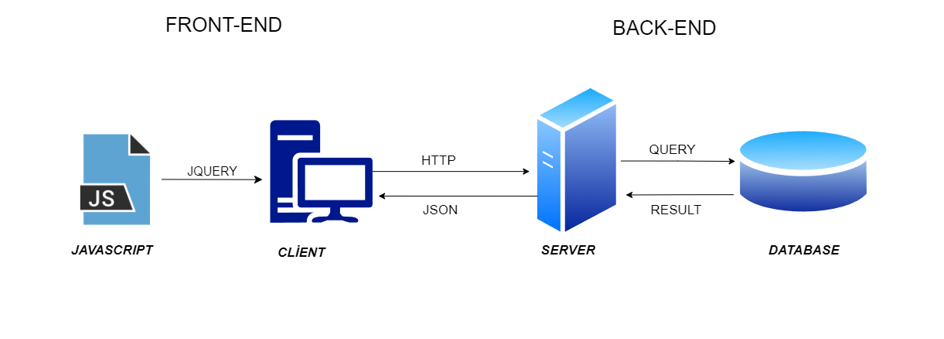
\includegraphics[width=\textwidth,keepaspectratio]{isleyis.png}



Projenin 4 katmanlı bir yapıda olduğunu belirtmiştim. Katmanlarda sırasıyla bahsedecek
olursam öncelikle Javascript katmanından başlamak isterim. Javascript katmanında jquery ile
ajax ve isteği oluşturup bir olayın tetiklenmesini sağlıyorum. Bu olay tetiklemesi
sonucunda client bir http isteği gönderiyor. Bu http isteği server katmanında tetiklenen olaya göre
içerde bir sorguyu çalıştırıyor. Bu sorgu veri tabanına bağlanarak veri tabanında gerekli işlmeleri 
gerçekleşririp bir result dönüyor. Server katmanına gelen bu result json formatta client katmanına geliyor.
Bu projenin 4 katmanlı olmasını sağlayan durum web sayfasının server tarafından hazır halde gelmeyip javascript 
katmnaında dinamik olarak hazırlanıyor olmasından kaynaklıdır.


Server tarafında, projenin iş mantığını ve veri tabanı etkileşimini yönetmek amacıyla .NET CORE üzerinde yazıp ASP.NET MVC modelini kullancağım. MVC mimarisi, uygulamayı modülerleştirir ve işlevselliği katmanlara bölerek daha yönetilebilir bir yapı oluşturur. Model katmanı, veri tabanına erişim ve veri tabanı ilişkileri gibi veri işleme süreçlerini içerir. View katmanı, kullanıcının etkileşimde bulunduğu arayüzü temsil ederken, Controller katmanı, kullanıcı komutlarını alarak bu komutları işleyen ara bir katman olarak görev yapar. Bu sayede, sistemin hem veri tabanı yönetimi hem de iş mantığı daha düzenli ve modüler bir yapı kazanmasını sağlayacaktır.
Asp.Net MVC modeli hakkında araştırmalarda kullanılmıştır.\cite{sozerihayatimda}
\vspace{1\baselineskip} %


MVC mimarisini kullanırken aynı zamanda SOLID prensiblerine uygun sekilde
kod yazmayı planlıyorum. SOLID prensiblerinden bahsedecek olursam beş temel ilkeye 
dayanıyor. SOLID prensipleri, yazılım geliştirme sürecinde kodun okunabilirliğini, bakımını,
esnekliğini ve yeniden kullanılabilirliğini artırmak için önemlidir. Bu prensiplere uygun kodlar,
daha az hata içerir, daha kolay anlaşılabilir ve daha sürdürülebilirdir. \newline 
Bu ilkeler ile ilgili araştırmamı ... adresinden yapmış bulunmaktayım.\cite{turan2018solid}\newline 
Aynı zamanda [\url{https://chat.openai.com/c/d70b0aba-f98f-4fad-a808-5ec4815176d4} ile de yararlandım.]
\vspace{1\baselineskip} %



Frontend tarafında ise JavaScript kullanarak sayfaları dinamikleştirme işlevselliği eklemeyi planlıyorum. HTML ve CSS, kullanıcı arayüzünü tasarlamak ve düzenlemek için kullanılacaktır. Bu sayede, kullanıcılar kitapları daha etkileşimli bir şekilde listeleyebilecek, arayabilecek ve filtreleyebileceklerdir.

Bu proje, modern teknolojilerin entegrasyonunu kullanarak uygulama geliştirme sürecindeki önemli konulara odaklanmakta ve hem veritabanı yönetimi hem de web uygulaması geliştirme konularında öğrenmeye yönelik bir deneyim sunmaktadır. Bu seçilen teknolojiler, projenin amacına uygun olarak sistemin etkili bir şekilde işleyişini destekleyeceği fikrindeyim.


	\begin{landscape}
\begin{figure}[h]
	\caption{GANTT CHART}
	\centering
	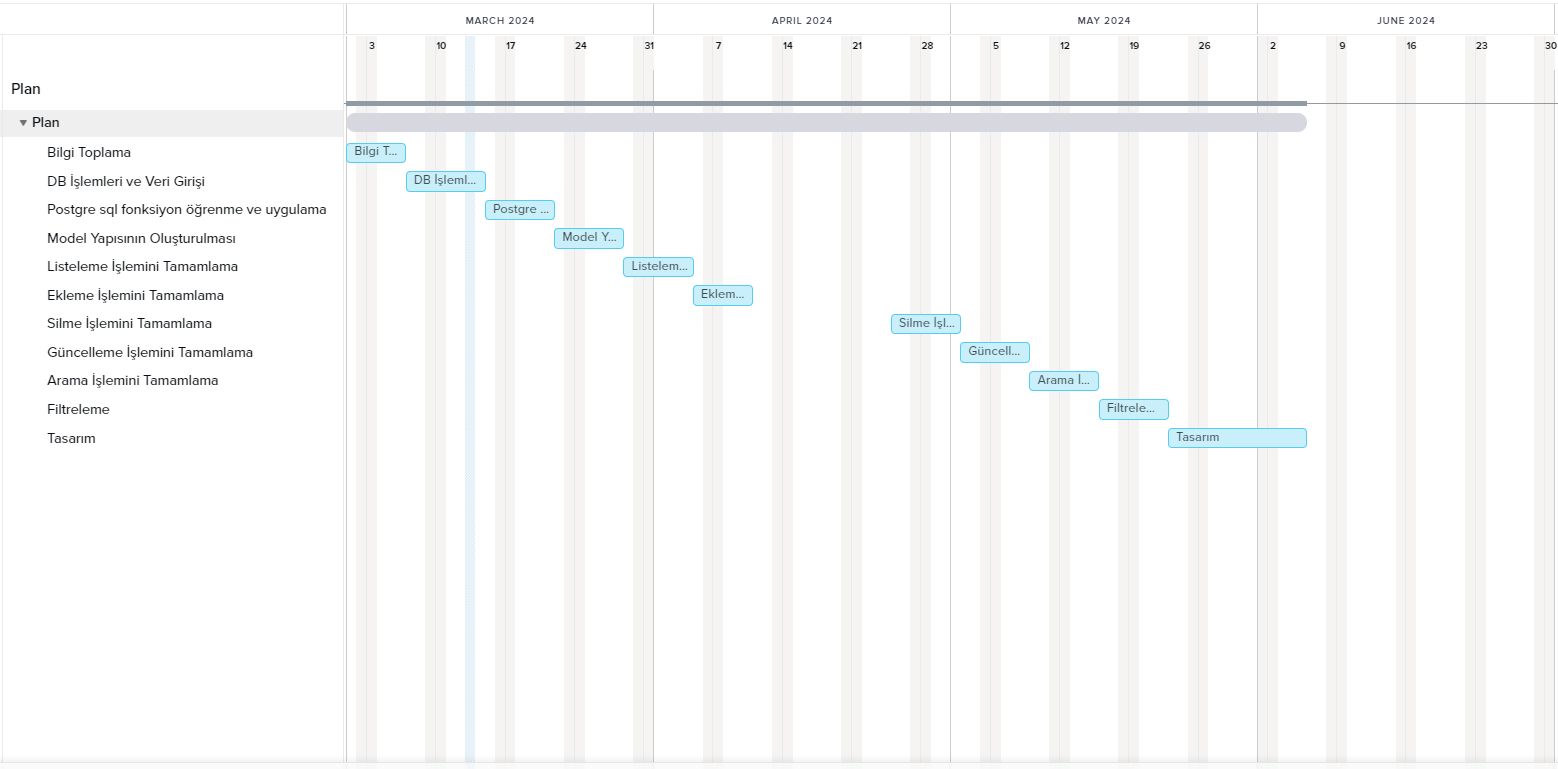
\includegraphics[width=\paperwidth,height=\paperheight,keepaspectratio]{plan.png}
	\label{gantt}
	Şekil  \ref{gantt}'de görebileceği üzere
	iş akış planı gösterilmektedir.
\end{figure}
\end{landscape}




\section{Veri Tabanı ve Veriler}	


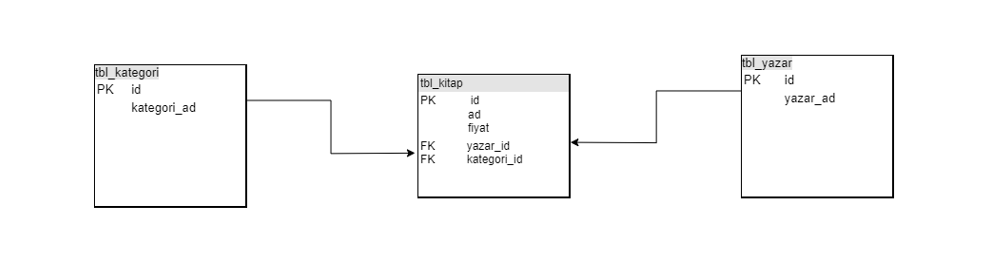
\includegraphics[ width=\textwidth]{tablolar.png} \newline



Database katmanında PostgreSQL'i tercih etmemin sebebi PostgreSQL'in açık kaynaklı yapısı ve lisans ücreti gerektirmemesi gibi avantajlarının olmasıdır.Çekirdek başına ve sürümüne göre maliyet diğer dillerde oldukça fazladır. PostgreSQL ile projede temel verileri depolamak için kullanılacak olan "kitap," "kategori," ve "yazar" gibi tabloları içermektedir.
Database işlemlerinde verinin kullanabilmesi için PostgreSQL fonksiyonlarından yararlanacağım.
\vspace{1\baselineskip} %
\newline

	PostgreSql fonksiyonları ile ilgili araştırmaları [\url{https://github.com/tubitak-bilgem-yte/pg-gelistirici.git}] adresinden gerçekleştirdim.\newline 
	
	\centering
	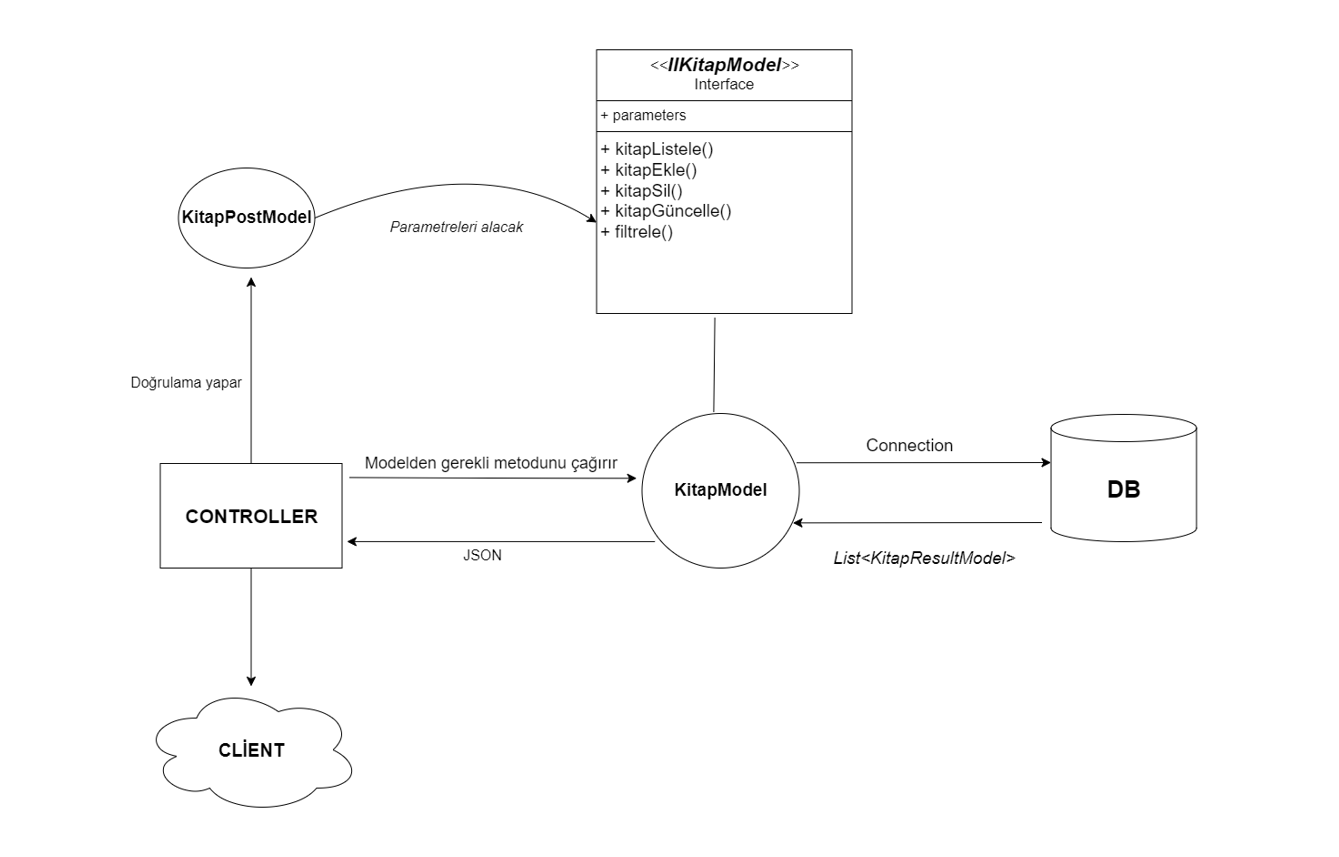
\includegraphics[ width=15cm, height=15cm,keepaspectratio]{Model.png} \newline


\begin{description}
	\item[\textbf{IKitapModel Arayüzü:}] Bu arayüz, kitaplarla ilgili işlemlerin sözleşmesini tanımlar. Yani, kitap listeleme ve kitap ekleme vb. işlevlerin prototiplerini içerir.Yapılacak işlemler için gerekli parametreleri KitapPostModel'den alır ve sonuç olarak bir KitapResultModel listesi döndürür.
	\item[\textbf{KitapModel Sınıfı:}] IKitapModel arayüzünü uygular (implement eder) ve bu arayüzde tanımlanan metodların somut davranışlarını içerir.
	PostgreSQL veritabanına bağlanır, bir SQL sorgusu çalıştırır ve sonuçları bir KitapResultModel listesine dönüştürür.
	Veritabanı bağlantısı ve sorgu işlemleri için NpgsqlConnection ve NpgsqlCommand nesnelerini kullanır.
	\item[\textbf{ KitapPostModel Sınıfı:}] Kullanıcıdan alınan verileri taşımak için kullanılır. Bu model,örneğin kitap listeleme işlemi sırasında kullanıcı tarafından sağlanan verileri (örneğin, bir kitap adı) içerir.
	\item[\textbf{KitapResultModel Sınıfı:}] Veritabanından dönen sonuçları temsil eder. Her bir KitapResultModel nesnesi, bir kitap kaydının id, ad, fiyat, yazarAd, kategoriAd gibi özelliklerini içerir.
	\item[\textbf{HomeController Sınıfı:}] MVC'nin Controller bileşenidir ve kullanıcı isteklerini yönetir.
	Index metodu, uygulamanın ana sayfasını döndürür ve genellikle kullanıcıya HTML içeriği sunar.	Örneğin kitapListe metodu, bir HTTP POST isteği ile çağrıldığında, KitapListePostModel tipindeki veriyi alır, modelin geçerliliğini kontrol eder ve KitapModel üzerinden kitap listesini çeker. Daha sonra bu listeyi JSON formatında istemciye (web tarayıcısına) geri döndürür.
\end{description}

\vspace{1\baselineskip} %

\begin{itemize}
	\item Kullanıcı, web arayüzünde bir eylem gerçekleştirir (örneğin, bir kitap listeleme isteği gönderir).
	\item İstemci tarafı kod (JavaScript), bu isteği HomeController'ın kitapListe metoduna POST olarak gönderir.
	\item HomeController, KitapListePostModel nesnesini alır ve doğrulama yapar.
	\item Doğrulama başarılıysa, KitapModel'in KitapListe metodunu çağırır ve veritabanından gerekli verileri çeker.
	\item Elde edilen veriler KitapResultModel listesi olarak dönüştürülür.
	\item Bu liste, JSON formatında istemciye geri gönderilir.
	\item İstemci tarafı JavaScript kodu, bu verileri alır ve kullanıcıya göstermek üzere işler.
\end{itemize}
	
	Asp.Net MVC model sınıfı hakkında araştırmalarda kullanılmıştır. \cite{kurtonline} \newline
\cite{ccelik2018oncul} \cite{tuzemen2014akademik} \cite{keskin2014facebook}

	


\section{Beklenen Sonuçlar}

Panelin, kullanıcıların kolayca erişebileceği ve etkileşimde bulunabileceği kullanıcı dostu arayüze sahip olması beklenmektedir . Bu, kullanıcıların kitap ekleme, düzenleme, silme gibi işlemleri hızlı ve verimli bir şekilde gerçekleştirebilmelerini  sağlayacaktır.\newline
Panelin, farklı kategorilerde kitapları yönetme yeteneği sağlaması beklenmektedir. Kullanıcıların kitapları başlık, yazar,  gibi özelliklere göre arama yapabilmeleri ve filtreleyebilmeleri gerekmektedir.\newline
Panelin, kullanıcıların kitap koleksiyonu içinde hızlıca arama yapabilmelerini sağlayacak gelişmiş arama ve filtreleme özelliklerine sahip olması beklenmektedir. Bu özellikler, kullanıcıların istedikleri kitapları kolayca bulmalarını sağlayacak şekilde tasarlanmalıdır.\newpage


	%Kaynakçayı yazdırmak
	\bibliographystyle{ieeetr}
	\bibliography{references.bib} 
	%\printbibliography %Prints bibliography
	
	
\end{document}